\section{Einleitung}
Im Zeitalter von Google, Amazon und Facebook ist das Thema Big-Data allgegenwärtig. So auch im Modul Fortgeschrittene Datenbanktechniken im zweiten Semester des Masterstudiengangs Verteilte Systeme. Im Rahmen eines Projekts sollte das Thema unter einer beliebigen Aufgabenstellung selbstständig untersucht und erarbeitet werden. Dabei haben wir uns für den Kaggle-Wettbewerb "`Acquire Valued Shoppers Challenge"', der im nächsten Abschnitt genauer beschrieben wird, entschieden. Bei der Umsetzung haben wir basierend auf dem Hadoop-Framework verschiedene Technologien wie beispielsweise MapReduce-Algorithmen kennengelernt.

\subsection{Aufgabenstellung}
Ziel unseres Projekts ist es, ein möglichst hohes Rating bei der "`Acquire Valued Shoppers Challenge\footnote{\url{https://www.kaggle.com/c/acquire-valued-shoppers-challenge}}"' zu erreichen.

Die Plattform Kaggle bietet Wettbewerbe im Bereich Big-Data an, bei denen statistische Analysen und Vorhersagemodelle erstellt werden sollen. Unternehmen und Forschungsinstitute können hier ihre Problemstellungen und die zugehörigen Daten zur Verfügung stellen, die von Statistikern und Data-Minern aus der ganzen Welt bearbeitet werden. Die Lösungen werden dabei nach ihrer Qualität, bezogen auf die Genauigkeit der Vorhersage, in einem Ranking bewertet und teilweise sogar prämiert. Damit bietet Kaggle den Aufgabenstellern die Möglichkeit, die beste der eingereichten Lösungsstrategien auszuwählen. Gleichzeitig können die am Wettbewerb teilnehmenden Teams die Qualität ihrer Lösung mit denen der Konkurrenz vergleichen.

Der Wettbewerb "`Acquire Valued Shoppers Challenge"', für den wir uns entschieden haben, beschäftigt sich mit der Fragestellung, ob Kunden die in der Vergangenheit Gutscheine verwendet haben, zukünftig weitere Produkte kaufen werden. Für die Lösung muss ein Vorhersagemodell erstellt werden, das für jeden Kunden die Wahrscheinlichkeit eines erneuten Kaufs vorhersagt. 

\newpage
\subsection{Projektmanagement}
Unser Projekt unterteilt sich insgesamt in folgende drei Phasen:

\begin{figure}[H]
\centering

\includegraphics[width=0.8\linewidth]{Bilder/ProjektplanAllgemein}
\caption{Die drei Projektphasen}
\label{fig:ProjektplanAllgemein}
\end{figure}

Im ersten Schritt der Einarbeitungsphase (Abb. \ref{fig:ProjektEinarbeitung}) soll eine Arbeitsumgebung in Form einer virtuellen Maschine (VM) ausgewählt werden. Anschließend wollen wir uns für ein konkretes "`Big-Data-Projekt"' entscheiden und das zugehörige Datenmodell analysieren. Im nächsten Schritt machen wir uns Überlegungen zu möglichen Data-Mining-Verfahren und legen uns auf geeignete Verfahren fest. Darauf basierend wird die Phase mit einer Technologieentscheidung zur Umsetzung des Projekts abgeschlossen.

\begin{figure}[h]
\centering

\includegraphics[width=1\linewidth]{Bilder/ProjektEinarbeitung}
\caption{Die Einarbeitungsphase}
\label{fig:ProjektEinarbeitung}
\end{figure}

Die Implementierungsphase (Abb. \ref{fig:ProjektImplementierung}) soll iterativ gestaltet werden und mit einer initialen einfachen Umsetzung beginnen. Basierend auf der ersten Implementierung wollen wir uns stetig verbessern. Im Zuge der iterativen Verbesserungen soll der Umstieg auf die Amazon-Web-Services vollzogen werden. Zur Bewertung der Zwischenergebnisse beenden wir jede Iteration mit der Einreichung des aktuellen Zwischenergebnisses bei Kaggle. Mit Abgabe der finalen Implementierung wollen wir aus der Implementierungsphase in die Abschlussphase (Abb. \ref{fig:ProjektAbschluss}) übergehen.

\begin{figure}[h]
\centering
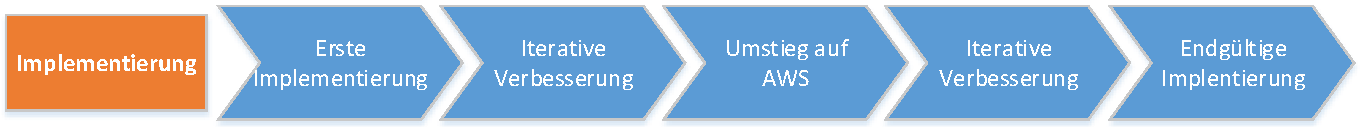
\includegraphics[width=1\linewidth]{Bilder/ProjektImplementierung}
\caption{Die Implementierungsphase}
\label{fig:ProjektImplementierung}
\end{figure}

In der Abschlussphase reichen wir das finale Ergebnis ein. Anschließend wollen wir die Projektdokumentation fertigstellen und unsere Erkenntnisse im Rahmen einer Abschlusspräsentation aufbereiten. Nach der Benotung lassen wir das Projekt in gemütlicher Atmosphäre ausklingen.

\begin{figure}[h]
\centering
\includegraphics[width=1\linewidth]{Bilder/ProjektAbschluss}
\caption{Die Abschlussphase}
\label{fig:ProjektAbschluss}
\end{figure}
